\section{准备工作} \label{sec:preparation}

本文假设小伙伴已经正确安装了 \TeX~Live 并对个人爱好的编辑器进行了相应的配置。安装与配置可以参考我博客里的\href{https://ichunyu.github.io/categories/latex/}{系列文章}。Elsevier 的模板已被该发行版收录,且本文所需的其他所有宏包均无需再手动下载。


\LaTeX 在编译过程中会产生大量的临时文件,通常由独立的文件夹来管理不同文档。对于期刊文章这类小型文档,个人推荐的文件结构由以下5部分构成:

\begin{itemize}
    \item 顶层设置文件

        类似与各类程序的主函数,建议使用独立的 \verb|.tex| 文件管理文件结构。在该顶层文件中对期刊模板进行设置,例如文章标题、作者、地址等信息。此外,顶层文件还对修订过程中临时使用的宏包进行设置,并利用 \verb|\input| 命令引入正文所需的宏包以及正文内容、管理致谢、参考文献等章节的基本顺序。这样做的好处在于:不同期刊提供了不同的模板,当需要更换不同期刊模板时,只需要创建新的顶层文件并进行相应修改即可。本文的顶层文件为 \verb|ElsevierPaper.tex|。

    \item 正文内容文件

        使用独立的文件编写正文内容,有利于将内容与格式分离。文章的所有内容(从引言开始)都汇总在单个文件中,在后续需要修订时,只需要编辑正文文件即可。同时,如果手动进行版本控制,只需要对正文文件进行备份,而不需要备份整个文件夹。本文的正文内容文件为 \verb|main.tex|。

    \item 宏包设置文件

        使用独立的文件单独管理正文所需的宏包,并进行相应设置。这样的好处是在更换模板时可以直接引入之前的配置,而不必对正文内容重新进行配置。本文的宏包设置文件为 \verb|packages.tex|。

    \item 参考文献数据库

        正文所应用的参考文献及其相关信息汇总在独立的 \verb|.bib| 数据库文件中,该文件通常可以通过外部文献管理软件导出。本文的参考文件数据库为 \verb|references.bib|。

    \item 图片文件夹

        正文可能会插入多个图片,可汇总在单独的文件夹内。本文的图片文件夹为 \verb|figures/|。
\end{itemize}


本文尽可能采用干净的代码风格,旨在帮助读者将本文与其源码相结合,更快地熟悉 \LaTeX 文档编写规则。同时,读者可直接基于本模板进行文章的编写,完成后依据顶层文件的注释删除汉化设置即可。


\TeX~Live 收录了 \verb|latexmk| 脚本,可用于自动编译文档。当正文包含中文时(注释除外),应使用 \verb|latexmk -xelatex ElsevierPaper.tex| 进行编译(注意替换顶层文件的名字);否则通常会使用 \verb|latexmk -pdf ElsevierPaper.tex|。特别地,如果在上述命令中进一步添加 \verb|-pvc| 选项,该脚本将会在后台运行并监测文件改动。当文件保存时会自动编译。如此做,如果保存的文件包含错误命令,后台的 \verb|latexmk| 脚本会暂停,需要在命令行的提示处输入 \verb|R| 使其重新启动,或输入 \verb|X| 退出脚本。




\section{标题与模板设置} \label{sec:frontmatter}

由于不同的期刊模板会提供不同的命令进行标题页设置,所以标题页通常建议在顶层文件进行设置。可以通过命令行运行 \verb|texdoc elsarticle| 查看 Elsevier 模板的官方说明,或打开本文的顶层文档跟我一起进行配置。


首先通过 \verb|\documentclass| 命令声明文档类,并在花括号中指明 Elsevier 模板,这样就完成了文章绝大部分的格式设置。进一步,可以使用中括号对文档类进行细部设置,例如对双盲审期刊,可在投稿时加入 \verb|doubleblind| 选项隐藏必要信息。除此外,这里介绍该模板支持的三种文档格式,其他可选项请参考官方说明。

\begin{itemize}
    \item \verb|1p|:正文在 $\SI{13.5}{cm}\times\SI{19.75}{cm}$ 范围内,且只能使用单栏排版;
    \item \verb|3p|:正文在 $\SI{16.45}{cm}\times\SI{21.9}{cm}$ 范围内,可使用单栏或双栏排版;
    \item \verb|5p|:正文在 $\SI{18.35}{cm}\times\SI{24}{cm}$ 范围内,且只能使用双栏排版;
\end{itemize}


本文使用了 \verb|[3p,onecolumn]| 选项,读者可尝试将第二选项改为 \verb|twocolumn| 转化为双栏。应当注意,\verb|1p| 和 \verb|5p| 格式不需要指定分栏样式。


声明文档类后,使用 \verb|\usepackage{hyperref}
\hypersetup{hidelinks}
% \hypersetup{colorlinks}

\usepackage{amsmath}
\usepackage{newtxmath}
\usepackage{bm}

\usepackage{siunitx}

\usepackage{enumitem}
\usepackage{graphicx}
\usepackage{booktabs}
\usepackage{subcaption}
\graphicspath{
    {./figures/}
}

% Caption Style
\usepackage{caption}
\captionsetup{labelsep=period}

\usepackage[capitalise,nameinlink]{cleveref}
\usepackage{tocbibind}
| 导入正文所需的宏包。这些宏包通常只是对部分功能进行美化,将在\cref{sec:context}进行介绍。


紧接着的三个命令分别是 \verb|\journal| 指定投稿期刊、\verb|bibliographystyle| 使用 Elsevier 的参考文件样式、\verb|biboptions| 将参考文献设置为按顺序编号并压缩连续引用的编号。


修订格式的设置将在\cref{sec:revision}进行介绍,这里暂且跳过。需要注意的是,修订部分的格式只在与审稿人沟通时显式标记修改。如果期刊要求最终提供干净的源码,这部分格式设置将是不必要的。因此放置在顶层文件中随时注释以取消设置。


Elsevier 期刊模板只适用于英文,本文的中文魔改主要依赖于 \verb|ctex| 宏包,相关设置不予介绍。基于本文源码编写英文文档时,完成后应当将中文魔改部分删除或注释。


在 Elsevier 模板中,标题页的所有设置均在 \verb|frontmatter| 环境中完成,且该模板提供的命令大多都是可以顾名思义的:使用 \verb|\title| 声明文章的标题,使用多个 \verb|\author| 按顺序给出作者。其中,\verb|\author| 可使用中括号作为可选项指定作者的地址,中括号内的数字编号与后面定义通讯地址的 \verb|\address| 或 \verb|\affiliation| 的数字编号相对应。其中,\verb|\address| 需要手动分割各级地址的信息,而 \verb|\affiliation| 采用键值对的方式录入地址。文章的通讯作者可以使用 \verb|\corref| 和 \verb|\cortext| 这一对命令指定,前者需要放置在 \verb|\author| 命令内,后者一般显示地标记“通讯作者”字样并给出邮箱信息。




\section{编写文档} \label{sec:context}

\subsection{正文} \label{subsec:text}

在 \LaTeX 文档中,正文的绝大部分内容都以文本的形式呈现。正文文本的换行不会引起编译后文档的换行,这使得在修改时不必完全删除之前的内容,只需要将被修改的内容换行并注释掉即可。
% 比如这里就注释掉了一句不需要出现在正文中的句子。
% 并且只要不出现空行,就不会导致实际文档的换段。
需要进入下一段时,源码的两段文字之间要求至少存在一个空行。


为了区分正文的章节,可以使用 \verb|\section|、 \verb|subsection| 或 \verb|\subsubsection| 命令分节,并给出各节的小标题。这些命令可以增加星号,如 \verb|\section*|,这样产生的新的一节不会进行编号,常用于致谢和参考文献。


对于理工学科,正文中通常会出现带单位的数字,例如 \SI{e5}{km}。使用 \verb|siunitx| 宏包的 \verb|\SI| 命令可以很方便地处理这类问题。该命令的第一个参数为数值,支持程序语言的写法如 \verb|5.2e-15|,第二个参数为单位。该命令可以自动处理数值与单位之间的空格以及单位的直立字体。特别地,该宏包支持使用国际单位制的标准单位,例如 \verb|\SI{10}{\micro\meter}| 将编译成 \SI{10}{\micro\meter}。特别地,角度可以简单地使用 \verb|\ang{90}| 命令,对应的输出为 \ang{90}。


\subsection{插图} \label{subsec:figures}

一般的插图可以结合 \verb|figure| 环境和 \verb|\includegraphics| 命令来完成,由于我们将图片汇总在一个文件夹内,为了省略插图使的路径,可以在宏包设置中使用 \verb|\graphicspath| 设置搜索路径。


\begin{figure}[!htb]
    \centering
    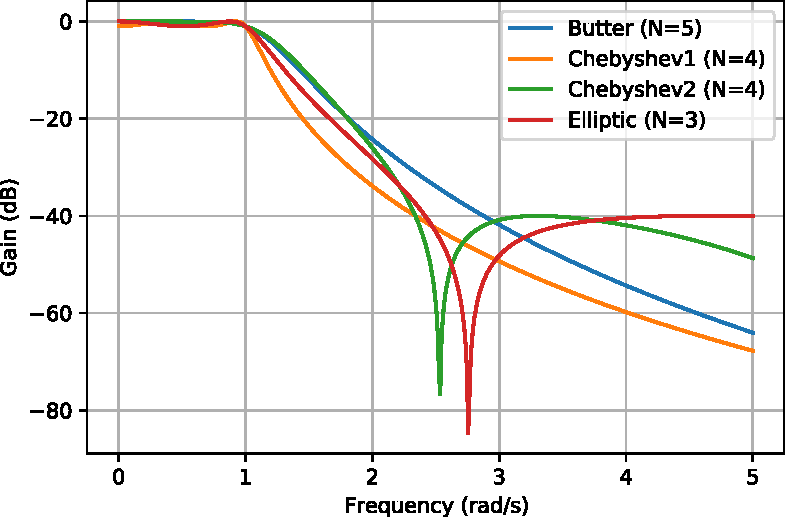
\includegraphics[width=70mm]{filter.pdf}
    \caption{常用滤波器幅频响应对比}
    \label{fig:filter}
\end{figure}


\cref{fig:filter} 给出了一个插图的示例。结合源码:\verb|figure| 环境后的 \verb|[!htb]| 表示图片可以根据源码中上下文的关系出现在相应位置(\verb|h|),或放置在页面的顶端(\verb|t|)或底端(\verb|b|)。感叹号表示放松 \LaTeX 的排版约束。


插图时可以手动指定图片的宽度,图片会按照比例进行缩放。图片的常用格式包括 \verb|.png|、\verb|.jgp|、\verb|.eps|、\verb|.pdf| 等,前两种是位图格式,后两种为矢量图。使用矢量图可以避免放大时模糊。插图之后使用 \verb|\caption| 定义图名,并使用 \verb|label| 打上标签,用于交叉应用。


特定情况下可能需要图片并列排版,并以子图的形式呈现,这可以通过 \verb|subcaption| 宏包实现,如\cref{fig:FilterCompare} 所示。该宏包提供的 \verb|\subcaptionbox| 命令依次接收子图图名和插图命令。通过在子图的图名之后打上标签,也可以对子图进行引用,如\cref{fig:prjFilter}。由于子图并排占据了较大的排版宽度,在双栏模式下可能会被强制换行。如果希望保持并排的样式,可以将 \verb|figure| 环境改为 \verb|figure*|。


\begin{figure*}[!htb]
    \centering
    \subcaptionbox{切比雪夫II型滤波器幅频响应\label{fig:prjFilter}}{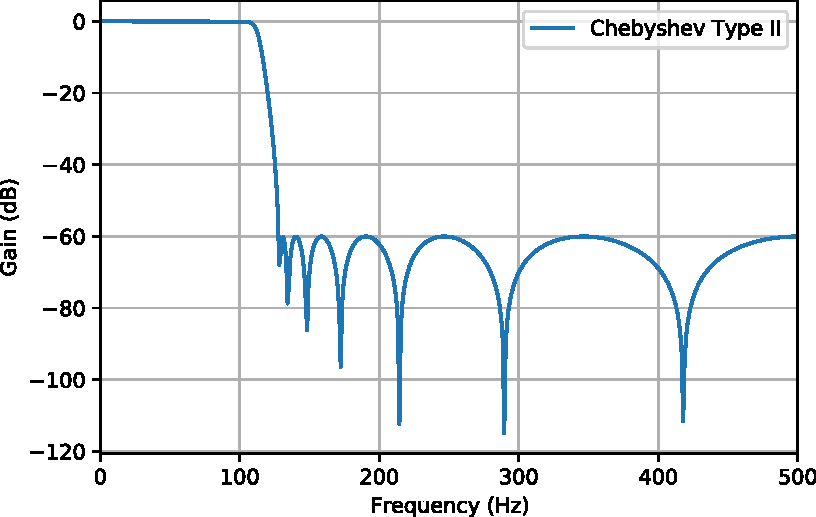
\includegraphics[height=40mm]{prjFilter.pdf}}
    \hspace{5mm}
    \subcaptionbox{零相位滤波与直接滤波时域对比\label{fig:ZeroPhaseFiltering}}{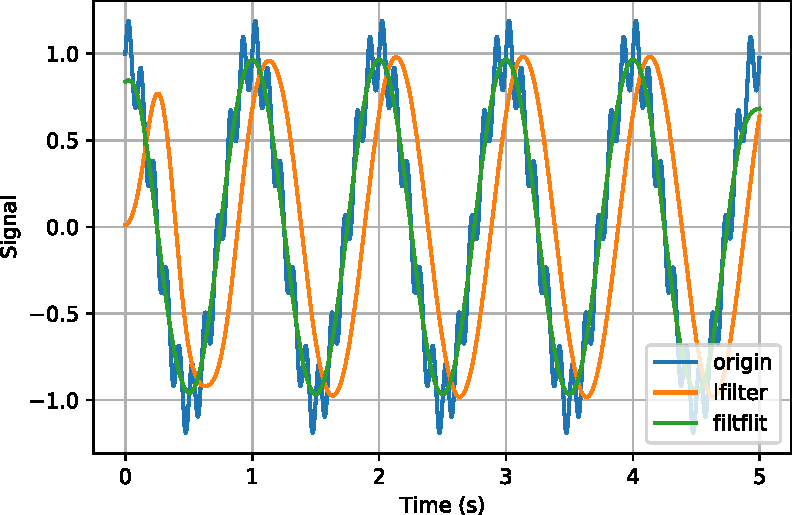
\includegraphics[height=40mm]{ZeroPhaseFiltering.pdf}}
    \caption{滤波器幅频响应与滤波效果对比}
    \label{fig:FilterCompare}
\end{figure*}


\subsection{表格} \label{subsec:tables}

表格可以使用 \verb|table| 环境结合 \verb|tabular| 构成表格,如\cref{tab:packages} 所示。表名和标签的设置与插图非常类似,只是表名通常在表格之前,顺序进行了调整。\verb|tabular| 后的参数为各列的对齐方式,通常使用左对齐(\verb|l|),相应地还有居中对齐(\verb|c|)和右对齐(\verb|r|)。需要注意的是,这里的设置应当与列数相一致,否则编译时会产生错误。


\begin{table}[!htb]
    \centering
    \caption{本文正文涉及的必要宏包}
    \label{tab:packages}
    \begin{tabular}{ll}
        \toprule
        宏包              & 功能简介 \\
        \midrule
        \verb|hyperref|   & 生成超链接并处理超链接格式 \\
        \verb|amsmath|    & \AmS 数学宏包 \\
        \verb|newtxmath|  & 数学罗马字体 \\
        \verb|bm|         & 数学符号加粗 \\
        \verb|siunitx|    & 处理国际单位制 \\
        \verb|graphicx|   & 在正文中插图 \\
        \verb|booktabs|   & 绘制三线表的横线  \\
        \verb|subcaption| & 子图排版 \\
        \verb|caption|    & 设置图表名格式 \\
        \verb|cleveref|   & 自动处理交叉引用 \\
        \verb|tocbibind|  & 将参考文献加入 \verb|.pdf| 文件标签 \\
        \bottomrule
    \end{tabular}
\end{table}


期刊文章常使用三线表,借助 \verb|booktabs| 宏包可以轻松实现不同宽度横线的绘制,分别为:顶部横线 \verb|\toprule|,中间分割线 \verb|\midrule| 和底部横线 \verb|\bottomrule|。特别地,如果希望只绘制部分单元格下的分割线,可以使用例如 \verb|\cmidrule{2-5}| 命令在第二列到第五列绘制横线。


\subsection{公式} \label{subsec:equations}

\LaTeX 对数学的支持非常友好,然而很多初次接触 \LaTeX 的小伙伴可能不熟悉数学公式的代码。幸运的是,很多数学编辑软件都提供了 \LaTeX 代码转换的功能,不仅如此,还可以使用在线工具辅助编辑数学公式。例如我常用这个\href{https://www.latexlive.com}{妈叔的在线 \LaTeX 编辑器}。


\verb|amsmath| 宏包提供了扩展了很多数学环境,最常用的有:

\begin{itemize}
    \item \verb|equation|:单行公式,且能够自动编号,例如:
        \begin{equation}
            \sin 2 \theta = 2\sin\theta\cos\theta \label{eq:sin2theta}
        \end{equation}

   \item \verb|gather|:可以使用 \verb|\\| 换行的多行公式,每行自动编号,且各行居中对齐,例如:
       \begin{gather}
           \sin \left( \alpha + \beta \right) = \sin\alpha\cos\beta + \cos\alpha\sin\beta \label{eq:sinab} \\
           \cos \left( \alpha + \beta \right) = \cos\alpha\cos\beta - \sin\alpha\sin\beta \label{eq:cosab}
       \end{gather}

    \item \verb|align|:多行公式,每行自动编号,默认居中对齐,可使用 \verb|&| 手动指定对齐位置,例如:
        \begin{align}
            \cos2\theta &= 2\cos^2\theta-1 \label{cos2theta1}\\
                        &= 1-2\sin^2\theta \label{cos2theta2}
        \end{align}

    \item \verb|aligned|:多行公式子环境,通常与 \verb|equation| 一起使用,使多行公式只有一个编号。
        \begin{equation}
            \left\lvert x \right\rvert =
            \left\{
            \begin{aligned}
                x, &\quad x \le 0 \\
                -x, &\quad x < 0
            \end{aligned}
            \right.  \label{eq:abs}
        \end{equation}
\end{itemize}


\subsection{引用} \label{subsec:citations}

借助 \verb|cleveref| 宏包,交叉应用可统一地使用 \verb|\cref| 命令。为了能够正确应用,需要在适当的位置通过命令 \verb|\label| 打上标签。例如,我在这一节的开头使用 \verb|\label{subsec:citations}| 打上了标签,那么 \verb|\cref{subsec:citations}| 命令将会像这样产生对\cref{subsec:citations}的引用。在 \verb|hyperref| 宏包的加持下,交叉应用会以超链接的形式存在,并且由不同颜色的方框标识。这样可能会让文档看起来不够美观,为此我们可以使用 \verb|\hypersetup{colorlinks}| 将方框取消,通过改变字体的颜色来标记交叉应用。在本文的宏包设置中,我使用 \verb|\hypersetup{hidelinks}| 隐藏了超链接的颜色,以便与\cref{sec:revision}将要介绍的文档修订的颜色标记进行区分。


为了应用参考文献,需要事先准备 \verb|.bib| 文件,这通常可以从文献的主页导出,或者从文件管理软件中批量导出。该文件内的每一个题录通常以 \verb|@类别{键| 开头,利用\verb|\cite{键}| 就可以引用参考文献,例如随便引用一篇文献\cite{ObservationGravitationalWaves2016},引用多个参考文献时编号会聚合\cite{ObservationGravitationalWaves2016,SubFemtogFreeFall2016,LISALaserInterferometer1998}。为了能够正确编译出参考文献列表,一般在文章的最后使用 \verb|\bibliography{bib文件}| 指定参考文献列表的输出位置(不要 \verb|.bib| 后缀)。通常我会把这一声明放在顶层文件的最后。这样做的目的在于,如果必须通过手动调整部分参考文献的格式,我可以先进行编译,将生成参考文献的代码复制到单独的 \verb|.tex| 文件并进行修改,最后使用 \verb|\input| 插入参考文献代码来代替 \verb|\bibliography{bib文件}|。


\section{修订文档} \label{sec:revision}

投稿时根据期刊的要求,可能会需要在文中添加行号,这只需要引入 \verb|lineno| 宏包即可,并在开始编号的位置加上 \verb|\linenumbers| 命令即可。该宏包默认使用连续编号,如果希望每页重新编号,在引入宏包时加入 \verb|pagewise| 选项即可。在某些环境中行号会受到限制,例如该模板的 \verb|abstract| 环境。这时可以使用 \verb|linenumbers| 环境。


在文章修订过程中,通常要求显示地批注修订的内容,利用 \verb|changes| 宏包可以非常容易地实现该功能。使用 \verb|\added| 命令可以添加内容并以颜色进行标记;使用 \verb|\deleted| 可以标记删除的内容。特别地,\verb|\replaced| 命令的两个参数分别是修改后和修改前的内容,相当于前面两个命令的合体。根据我自己的经验,建议避免使用 \verb|replaced| 命令:一方面可以手动指定删除和新增的先后顺序,使修订的内容看起来更加连贯;另一方面,如果期刊最后要求提供干净的源码,利用正则表达式可以很轻松地处理掉 \verb|added| 和 \verb|deleted| 命令。如果期刊只需隐藏修订的 \verb|.pdf| 文件,只需要在导入宏包时加入 \verb|final| 选项即可。改宏包还提供了其他命令,相见其帮助文档。


需要注意的是,某些宏包或者模板可能提前定义了 \verb|\comment| 命令,这会导致使用 \verb|changes| 宏包时出现重复定义的错误。为此,在导入该宏包之前可以使用 \verb|\undef| 取消之前的定义。\verb|changes| 宏包可以自定义修订的标记,包括颜色、删除线等。如果没有特别的要求,通常可采用默认值。我个人习惯将删除的内容用灰色(浅色)标记,因此进行了相应的设置,仅供参考。


由于审稿人通常是义务劳动,必要时可以使用边注提醒审稿人修订的位置。在顶层文件的源码中我定义了 \verb|Rev| 命令,最后用一段废话来展示修订的效果:


这段话是一段用来展示修订效果的废话。比如审稿人 1 的第 1 个建议是将后面句话改为“把”字句:\Rev{1.1}\added{我吃了把鸡蛋}\deleted{鸡蛋被我吃了}。为了凑点字数以便与区分另一个审稿人的意见,我不得不再写这么一句废话。假如审稿人 2 的第 3 个意见是增加一点描述\Rev{2.3}\added{,那么修订后的句子应该是这个样子}。


\section{结语}

祝大家早日发文章,早日毕业!
